
\begin{defn}
  \label{defn:ReceptiveField}
  %The position of a sensory neuron’s input terminals in the sense organ is a major component of the specific information conveyed by that neuron.
  The skin area, location in the body, retinal area, or tonal domain in which stimuli can activate a sensory neuron is called its \emph{receptive field}.
  %The region from which a sensation is perceived to arise is called the neuron’s \emph{perceptive field}. The two usually coincide.
\end{defn}
\begin{rem}
  The following figure is the receptive field of a touch-sensitive neuron, which denotes the region of skin where gentle tactile stimuli evoke action potentials in that neuron. Sometimes receptive fields would change over time.
  \begin{center}
    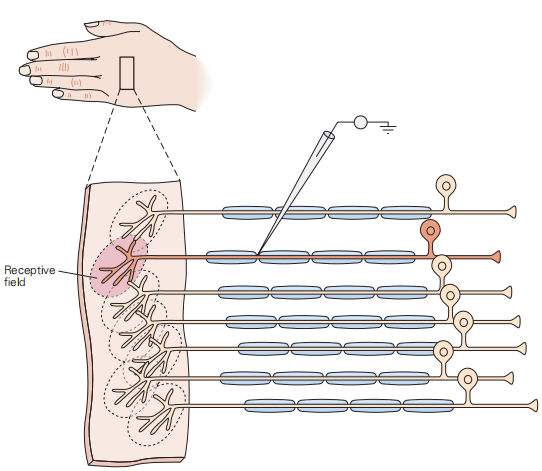
\includegraphics[scale=0.3]{./png/touchRecept}
  \end{center}
\end{rem}

%\begin{rem}
 % The spike-triggered average stimulus introduced in chapter 1
  %is a standard way of characterizing the selectivity of a neuron.
%\end{rem}

\begin{defn}
  \label{defn:reverse-correlation}
  \emph{Reverse-correlation} is a technique for studying
  how sensory neurons add up signals from different locations
  in their receptive fields, and also how they sum up stimuli
  that they receive at different times, to generate a response.
\end{defn}

\begin{rem}
  The goal of the reverse-correlation technique is to find a function $r = f(s)$ that maps from the stimulus $s$ to the neuronal response $r$, where the stimulus is a function dependent on spatial location and time $s = s(x,y,z,t)$. 
\end{rem}

\begin{rem}
  The reason that this technique is called "reverse" is that we align the time origin with the neuron's response and then reverse the timeline to find what stimulus ($t<0$) triggered the neuron's response at the current moment ($t=0$).
\end{rem}


%\begin{defn}
 % \label{defn: typesOfModels}
  %\emph{Descriptive Models} approximate descriptions of neural responses, and do not explain how visual responses arise from the synaptic, cellular, and network properties of neoral circuits. Nevertheless, they provide an important framework for characterizing response selectivities, a reference point for identifying and characterizing novel effects, and a basis for building mechanistic models, some of which are discussed at the end of this chapter.
%\end{defn}

\begin{asm}
  \label{asm:stimulus}
  As discussed in chapter \ref{cha:Neural Encoding I}, sensory systems tend to adapt to the absolute intensity of a stimulus. We therefore assume throughout this chapter that the stimulus parameter $s(t)$ has been defined with its mean value subtracted out, that is,
  \begin{equation}
    \label{equ:adaptionAssumption}
    \frac{1}{T}\int_0^Ts(t)dt = 0.
  \end{equation}
\end{asm}

%%% Local Variables:
%%% mode: latex
%%% TeX-master: "../notesOnFluidMechanics"
%%% End:
